\documentclass[onecolumn]{article}
\hoffset=0in
\voffset=-.2in
\marginparwidth=0in
\marginparsep=0in
\oddsidemargin=0in
\topmargin=0in
\headheight=0in
\textwidth=470pt
\textheight = 620pt
\fontsize{12}{15}
\pagestyle{empty}
\usepackage{multicol}
\usepackage{cite}
\usepackage[colorlinks=true, linkcolor=blue, citecolor=blue, urlcolor=blue]{hyperref}
\usepackage{amsmath,amssymb}
\usepackage{mathptm,graphicx,rotate,color}
\newcommand{\bb}[1]{\mathbb{#1}}
\usepackage{cite}
\newcommand{\DO}{$\delta^{18}O$ }
\begin{document}
\section{Methods}
\indent We attempt to search the parameter space within the limits suggested by Paillard \cite{paillard} in hopes of better fitting the both the discrete and the ODEE models to the \DO data by using a genetic algorithm (GA) and covariance matrix adaption evolutionary scheme (CMA-ES) to evolve possible parameters. CMA-ES and GA are well-known and documented evolutionary algorithms for evolving real-valued vectors that minimize a particular fitness function when evaluated. For this investigation, we chose to minimize the root mean square error of the normalized model compared to the \DO data. \\
\subsection{Datasets}
\indent We obtained to necessary data sets for running our experiments. Our \DO data comes from Tiedermann et al. \cite{d18} as the result of analyzing an ice core sample taken from up to 273.80 m in 1986. A simple linear transformation is used to scale from depth to the age of the samples. The ice core sample was taken in the North Atlantic Ocean. While this may not be the exact dataset used by Paillard, we believe the data contained here should be sufficiently similar and relevant in our efforts to fit Paillard's models to historical climate behavior.\\
\indent We employ the same insolation dataset used by Paillard in \cite{paillard}; namely, we use the data provided by A. Berger in \cite{berger}. Berger obtains this curve representing the earth's atmospheric insulation about the latitude $65^{o}N$ by modeling the earth's rotation about the sun. His calculations account for such variables as the angle of the earth's axis from perpendicular to the sun, and eccentricity. This insolation curve acts as the forcing for our model.\\
\subsection{Models}
\indent Paillard \cite{paillard} suggests two models for obtaining the \DO curves from atmospheric insolation data. These models represent the transformations of three different glacial states: $i$ (interglacial), $g$ (mild glacial), $G$ (full glacial). Both models allow us to impose limits on the insolation, the ice volume that determines the glacial state, and the expected time spent in each glacial state. In both models, it is assumed that the only three possible transitions exists. A $i\rightarrow g$ (interglacial$\rightarrow$ mild glacial) transition occurs when when the insolation falls below a parameter $i_{0}$. A $g\rightarrow G$ (mild glacial $\rightarrow$ full glacial) transition occurs when a maximum ice volume $v_{max}$ is exceeded. Finally, a $G\rightarrow i$ (full glacial$\rightarrow$ interglacial) transition occurs when the insolation grows above a parameter. \\
\indent Paillard first suggests a discrete model for obtaining the \DO curve from insolation data. This model has four insolation parameters.  $i_{0}$ and $i_{1}$ represent the insolation values required for $i-g$ and $G-i$ transitions to occur, respectively. The other insolation parameters $i_{2}$ and $i_{3}$ identify a range of possible forcing values that would allow a $g-G$ transition to occur. A further parameter, $\tau_{g}$, is a time constant determining the minimum number of years for the model to spend in a mild glacial state. In an effort to reduce the search space, we adopt Paillard's assumption of $\tau_{g}=33$ kyr for our discrete model and attempt to evolve values for the parameters $i_{0}$, $i_{1}$, $i_{2}$, and $i_{3}$.\\
\indent An ODE model is also presented by Paillard, which is given by \[ \frac{dv}{dt}=\frac{v_{R}-v}{\tau_{R}}-\frac{F}{\tau_{F}} \] where $v$ is the ice volume, $v_{R}$ and $\tau_{R}$ are the volume and the time constants, respectively, corresponding to the glacial state. $\tau_{F}$ is a time constant associated with a forcing parameter $F$. The forcing parameter $F$ is given through a truncation of the insolation data described by \[ F=\frac{1}{2}(x+\sqrt{4a^{2}+x^{2}})\] with $x$ being the insolation and a tunable compression parameter $a$. $i_{0}$ and $i_{1}$ are the same as in the discrete model, and the other insolation parameters are omitted. Again, we reduce our search space by adopting the assumption presented by Paillard that $\tau_{i}=10$ kyr, $\tau_{g}=\tau_{G}=50$ kyr, $\tau_{F}=25$ kyr, and $a=1$. We attempt to provide good choices for the remaining insolation parameters $i_{0}$ and $i_{1}$.\\
\subsection{Evolutionary Algorithms}
\indent Both of the evolutionary algorithms we used are designed to search through the space $\bb{R}^{n}$ with a population of $n$ length real-valued vectors with each entry corresponding to a parameter in our model. Through common genetic mechanisms, like reproduction and mutation, we are able to evolve vectors representing potentially good parameter choices for the insolation parameters in each model to fit the \DO  data. Both algorithms require a fitness function with which to assess how well the parameter choices represented by an individual vector represent the \DO data through the models. We employ a fitness function which integrates the model and then attempts to minimize the root mean square error of the resulting time series compared to the true \DO data. This fitness function allows us to apply selection pressure on the populations of vectors that results in competition within the population to fit the \DO data the best.\\
\vspace{.25cm}\\
\noindent{\bf Covariance Matrix Adaption Evolutionary Scheme (CMA-ES)}\\
\indent CMA-ES is often a good initial choice of evolutionary algorithm for evolving real-valued vectors because the algorithm itself is not expensive and the algorithm often yields a reasonably good result after only a few generations. The algorithm begins with a uniformly distributed cloud of points in $\bb{R}^{n}$. Each point represents parameter choices for the models. We asses the fitness of each point and create a covariance matrix weighted by the fitness values. By taking the average of the fitness values, we can determine weighted center of the cloud of points, and we can determine a direction to move that point that will hopefully yield a better average fitness. Having relocated the average point, we create a new cloud of points around the average, however we now use the covariance matrix to determine how to distribute the individuals points. For example, if the population members all agree at a particular index, then they will have small covariances. This will caus!
 e the new cloud of points to be very narrow in that dimension since all of the population members are in agreement. On the other hand, if all of the individuals disagree in a particular dimension, then there will be large covariances representing a need to explore more in that dimension. Thus, the cloud of points should be wider in that dimension. We fix the number of generations to be 500 for our experiments. More information about CMA-ES can be found in \cite{suttorp}.\\
\begin{center}
	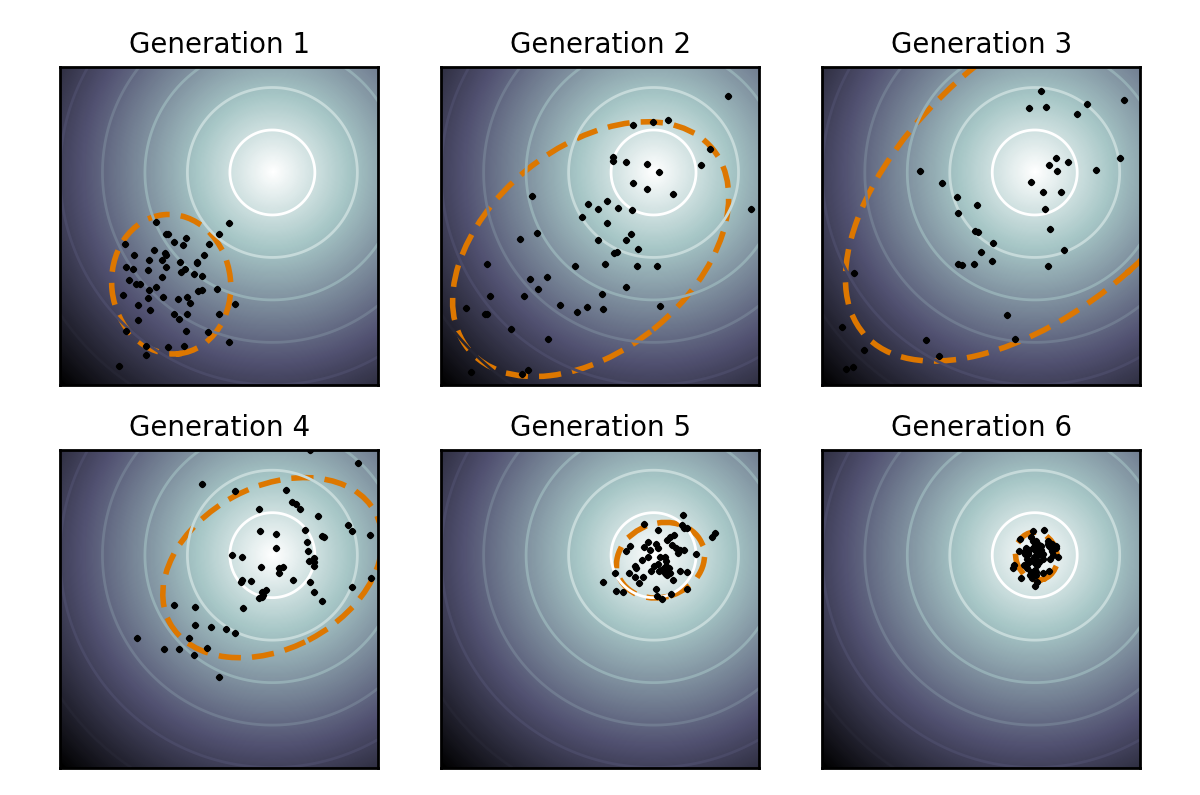
\includegraphics[scale=.6]{cmaes.png}
\end{center}
Figure 1. A cartoon representing 6 generations in a CMA-ES experiment. Here, lighter colors indicate improved fitness. The dashed lines represent the influence of the covariance matrix.\\
\vspace{.25cm}\\
\noindent{\bf Genetic Algorithm (GA)}\\
\indent GA's are typically more expensive than CMA-ES, but allow for an increased wealth in ways for population members to combine information. GA's often yield greater runtimes than CMA-ES but can also yield more robust explorations of parameter space. The algorithm begins with a population of real-valued vectors. Each vector is assessed for fitness. The fitter individuals in the population are chosen as candidates for reproduction in the form of crossover. Here, we use uniform crossover, which means that given two ``parent" vectors from the population, we create a ``child" vector by randomly selecting indices to contain the value stored in that index by parent 1. The remaining indices are filled with the values stored in parent 2 at those indices. A second child vector is created by taking the same random indices, and swapping the roles of the parents. These two children vectors then replace their parents in the population. Individuals in the population are also subject to!
  mutation. Mutation is performed on individuals where a small amount is added or subtracted from each index in an individual vector with some small probability. Crossover often leads the population to converge on good solutions, while mutation generally causes the population to explore parameter space. Striking a balance between these two forces is vital and often very difficult depending on the noise in the fitness landscape; that is, the fitness values associated with each point in the parameter space. For our experiments, we use a population size of 500 and calculate 500 generations.\\
\begin{center}
	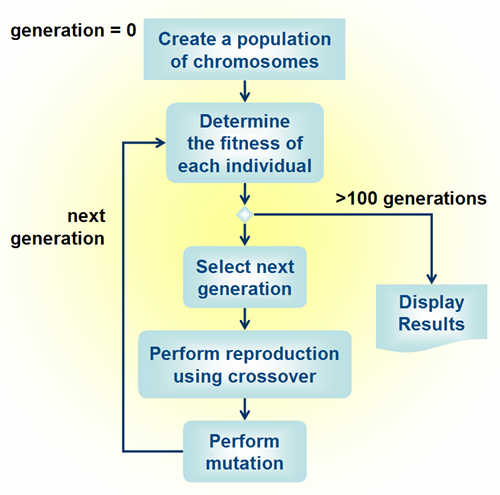
\includegraphics[scale=.6]{gaImg.png}
\end{center}
Figure 2. A schematic explaining the basic steps in a genetic algorithm.\\
\section{Results}
\indent Having run 100 CMA-ES and GA experiments, we discuss the fit of the best solutions here. Firstly, CMA-ES underperformed. None of the CMA-ES experiments yielded results worth noting here. This is likely due to unresolvable noise in the fitness landscape. We focus instead on the more promising results from our GA experiments.\\
\begin{center}
$\begin{array}{cc}
	\includegraphics[width=.5\columnwidth]{discrete}&\includegraphics[width=.5\columnwidth]{ode}
\end{array}$
\end{center}
Figure 3. {\bf (Left)} The best result from the GA experiments attempting to fit parameters to Paillard's discrete model. {\bf (Right)} THe best result from the GA experiments attempting to fit parameters to Paillard's ODE model. The root mean square errors are reported at the top. \\
\vspace{.25cm}\\
\indent Figure 3 demonstrates the results of our most promising GA experiments along with their root mean square errors (RMSE) from the \DO data. We should note that the particular parameter choices proposed by Paillard in \cite{paillard} yield RMSE$=1.42$ for the discrete model, and RMSE$=1.7186$ for the ODE model. Figure 3 shows that our GA experiment ($i_{0}= -0.7293$, $i_{1}=-0.2287$, $i_{2}=0.0803$, and $i_{3}=0.9862$) was only narrowly outperformed by Paillard's parameter choices for the discrete model, and that our GA experiment ($i_{0}= -0.9677$ and $i_{1}=0.0294$) yields a better fitting ODE model than the model suggested by Paillard's parameter choices for this model.\\
\indent 
\begin{thebibliography}{9}
	\bibitem{paillard}
	Paillard D. Laboratoire de Mod�lisation du Climat et de l'Environnement, CEA/DSM, Centre d'Etudes de Saclay, 91191 Gif-sur-Yvette, France
	\bibitem{d18}  Tiedemann, R et al. (1994): Stable oxygen isotope ratios of Cibicidoides wuellerstorfi from ODP Hole 108-659A in the North Atlantic. doi:10.1594/PANGAEA.52517,
        In Supplement to: Tiedemann, Ralf; Sarnthein, Michael; Shackleton, Nicholas J (1994): Astronomic timescale for the Pliocene Atlantic d18O and dust flux records of Ocean Drilling Program site 659. Paleoceanography, 9(4), 619-638, doi:10.1029/94PA00208
        \bibitem{berger} Berger, A. Long-term variations of daily insolation and Quaternary climatic change.J.Atmos. Sci. 35,
2362�2367 (1978).
	\bibitem{suttorp}
T. Suttorp, N. Hansen, C. Igel, Efficient covariance matrix update for
variable metric evolution strategies, Machine Learning 75 (2009) 167�
197
\end{thebibliography}
\end{document}